\chapter{Computing with Digital Information}
It is common knowledge that personal computers have become faster at
an incredible rate since they were first introduced in the mid-1970s.
But how fast are they, and how fast were they even five years ago?  A
quick Internet search leads us to the ``How Stuff Works'' Web page at
microprocessors\\
{\footnotesize{\texttt{http://computer.howstuffworks.com/microprocessor1.htm}}}\\
where we find the table shown in Figure~\ref{fig:HowStuffWorks}.  Run
your eyes down the columns of numbers and it's clear that the chips
have grown tremendously in terms of numbers of transistors, clock
speed, and MIPS.  But, it's difficult to see the rate of change,
e.g. Has the growth been exponential? Have these various measures
grown at the same rate?


\begin{figure}
\begin{center}
\begin{tabular}{c}
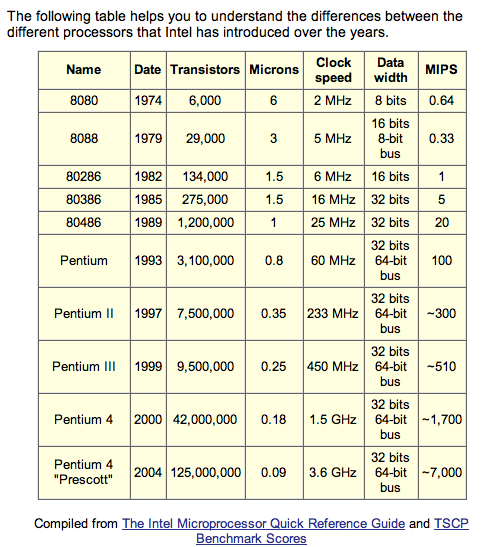
\includegraphics[width=5in]{computerIntro/images/howStuffWorks.png}
\end{tabular}
\caption{This screenshot taken from the ``How Stuff Works'' Web page
  {\footnotesize{\texttt{http://computer.howstuffworks.com/microprocessor1.htm}}}
  compares the various Intel chips since the 8080 chip was first
  introduced in 1974.  The Intel microprocessor has become much
  faster, smaller, and more powerful in the past thirty years, as seen
  by several measures.  From left to right, these measures are the
  number of transistors on the chip, the width in microns of the
  smallest wire on the chip, the clock speed (number of cycles per
  second), the number of bits used for addressing data in RAM, and the
  number of instructions processed per second (in millions).  The plot
  in Figure~\ref{fig:chip} shows a comparative picture of the changes
  in these variables over time.}
\label{fig:HowStuffWorks}
\end{center}
\end{figure}


To answer these questions, we need to get the data out of the Web page
in order to plot or compute rates of change from these measurements.
To extract the data, we could copy and paste from the browser into an
Excel spreadsheet or a plain text file, and then edit a bit to fix up
any errors made in the copy and paste.  Or, we could simply type the
numbers into Excel or a plain text file.  Table~\ref{tab:chip} and
Figure~\ref{fig:csvExcel} show the data in these new formats.  Neither
of these approaches are necessarily recommended because they are prone
to error, do not leave a trail of the process used to create the data,
and can be cumbersome if the process needs to be repeated in the
future (e.g. when a new processor is introduced).  Later chapters will
provide alternative ways to get data out of a table on the Web page
and into a format more conducive to further analysis.

\begin{table}
{\footnotesize{
\begin{verbatim}
Name       Date  Transistors Microns  Speed Units Data 	MIPS
8080       1974       6000     6        2   MHz    8       0.64
8088       1979      29000     3        5   MHz   16       0.33
80286      1982     134000     1.5      6   MHz   16       1
80386      1985     275000     1.5     16   MHz   32       5
80486      1989    1200000     1       25   MHz   32      20 
Pentium    1993    3100000     0.8     60   MHz   32     100
PentiumII  1997    7500000     0.35   233   MHz   32     300
PentiumIII 1999    9500000     0.25   450   MHz   32     510
Pentium4   2000   42000000     0.18     1.5 GHz   32    1700 
Pentium4x  2004  125000000     0.09     3.6 GHz   32    7000
\end{verbatim}
}}
  \caption{An alternative format for the data in Figure~\ref{fig:HowStuffWorks}: a plain text table, where the measurements are separated by blank spaces.}\label{tab:chip}
\end{table}

\begin{figure}
\begin{center}
\begin{tabular}{c}
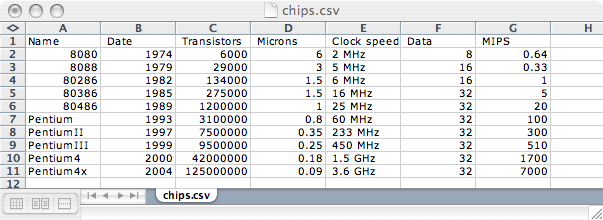
\includegraphics[width=5in]{computerIntro/images/excelScreenshot.png}
\end{tabular}
\caption{A screen shot of an alternative format for the data in
  Figure~\ref{fig:HowStuffWorks}: an Excel spreadsheet of the data.}
\label{fig:csvExcel}
\end{center}
\end{figure}

With the plain text file, we can easily read the data into the
statistical software R, and examine graphically the changes in the
number of transistors, the width of the smallest wire, the clock
speed, etc. of the Intel chip.  Figure~\ref{fig:chip} shows how the
Intel chip has experienced exponential growth according to all of
these measures, with the change in the width of the smallest wire
having the slowest growth (Note that it is the rate at which the
thickness has decreased which is plotted for this variable).  In a
way, it is not all that surprising that the other three measures are
very similar because clock speed and MIPS are directly related to the
number of transistors on the chip.

\begin{comment}
The code for preparing the data to make the plot appears below.  In
later chapters, we will cover the R statistical software in greater
detail, but for now notice that the five lines of code do the
following tasks: read in the data from a plain-text file; change the
values in Speed so that they all have the same units, i.e. MHz; select
the variables to be examined; normalize these variables by the value
in the initial year so the measurements become relative to 1974; and,
finally, invert the Microns measurement so it is increasing rather
than decreasing. Once the data have been transformed, they can be
plotted as in Figure~\ref{fig:chip}.
{\footnotesize{
\begin{verbatim}
chips = read.table("Chip.txt", header = TRUE, row.names = 1)
chips$Speed[ chips$Units == "GHz" ] = 
     1000* chips$Speed[chips$Units =="GHz"]
measures = c("Transistors", "Speed", "Microns", "MIPS")
chipsRate =  chips[measures]/as.numeric(chips[1, measures])
chipsRate$Microns = 1/chipsRate$Microns
\end{verbatim}
}}
\begin{verbatim}
matplot(chips$Date, chipsRate, 
  type="l",  log="y", lwd=2, lty=1, 
   ylab= "Growth in comparison to 1975 - log scale",
   xlab= "Date", col= c("black","red","green","blue"))

varl = names(chipsRate)
legend(1976, 1000, legend=varl, fill=coll, bty="n")

 abline(v=1993, col="grey")
  mtext(text="Pentium", side=3, line=-1.2, at=1993+0.1,adj=0)
 abline(v=1985, col="grey")
 mtext(text="32 bit processor", side=3, line=-1.2,at=1985+0.1,adj=0)
\end{verbatim}
\end{comment}

\begin{figure}
\begin{center}
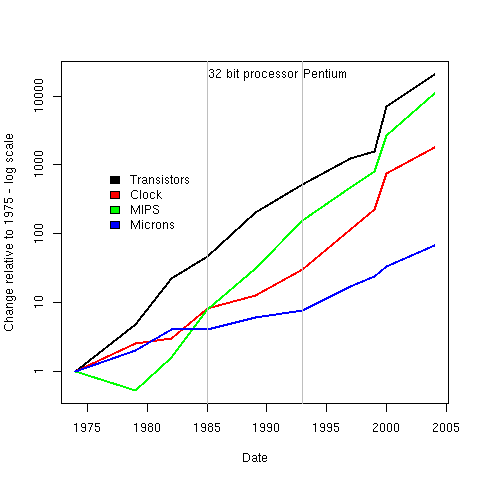
\includegraphics[height=4in]{computerIntro/images/bestChips.png}
\caption{This graphical display of the data from the plain-text table
  of values in Table~\ref{tab:chip} shows how the computational
  power of the Intel microprocessor has grown exponentially over the
  past thirty years. The grey lines mark the introduction of the
  32-bit processor and the Pentium processor in 1985 and 1993,
  respectively.}
\label{fig:chip}
\end{center}
\end{figure}

By now, you may be wondering: What is a microprocessor and what are
MIPS and Clock speed?  What is the difference between a table in a Web
page, an Excel spreadsheet, and a plain-text table?  What are these
computation in R doing?  These questions are important to
understanding basic notions in data technology.  One doesn't need to
be a techno-wizard to use a computer to analysze data, but there are
some fundamental concepts that can make a big difference in helping
you take full advantage of the tools available for handling data.
Addressing these questions are the topic of this chapter.

In Section~\ref{sec:computation} we introduce some terminology that we
use to describe computations and the basic syntax for carrying out
statistical computations in R.  This section leads into a brief
overview of the various types of computing languages, e.g. compiled
and interpreted languages, and examples of them
(Section~\ref{sec:languages}).  Next we examine how information, such
as text, numbers, and images are represented in a computer and how
they are organized into files and directories
(Section~\ref{sec:digital}).  The chapter concludes with a brief
description of basic the components of a computer
(Section~\ref{sec:components}). If you are already quite familiar with
these topics then you may want to skim this chapter.


\section{Computations}\label{sec:computation}
The instruction set on a computer chip provides the basic primitives
with which we can build more sophisticated, higher-level computations
to, for example, add a vector of numbers, sort a list of names, and
make a plot.  Whether primitive, complex, or high-level, a computation
acts on one or more inputs to create an output, and it can be thought
of as a transition from an old state to a new state: to add a set of
numbers, we take the various numbers as inputs and create one output
-- the sum; to sort a list of names, the input list of names
transitions to an alphabetically sorted list; and to make a plot of
the change in microprocessors in the past thirty years, the computer
acts on the data (Table~\ref{tab:chip}) to produce the image shown
in Figure~\ref{fig:chip}.

In general, we \Key{invoke} a computation with an
\Key{expression}. For example, the expression \RCode{17 + 100} is
handed off to the computer for \Key{evaluation}; the inputs, $17$ and
$100$, are acted on, and the \Key{return} value of the expression is
$117$.  The plus sign \RCode{+} is an \Key{infix operator}, meaning
that it comes between its inputs ($17$ and $100$).  The R language
uses both infix operators such as $+$, $*$, \verb+^+, $/$ for
addition, multiplication, exponentiation and division, respectively,
and it uses \Key{function style computations}.  Function style
computations in R have the general format,
\begin{verbatim}
functionName(argument, ... , argument)
\end{verbatim}
For example, \RCode{rnorm(3)} invokes the \RCode{rnorm} computation to
generate three random normal values. That is, the input to the
function \RCode{rnorm} is $3$, and the output is $3$ numeric values
that are randomly generated from the normal distribution.
\begin{verbatim}
-2.2994024 -0.4127883  0.1197349
\end{verbatim}

The arguments in a function-style computation can also be identified by
name.  The computation below provides the inputs $3$, $2$ and $1$ to
the computation in order to generate $3$ random values from a normal
distribution with mean $2$ and standard deviation $1$.
\begin{verbatim}
rnorm(3, mean = 2, sd = 1)
2.8913993 -0.4770861  2.7620108
\end{verbatim}
The details of the syntax for the R language are covered in greater
detail in Chapter~\ref{chap:RIntro}.

The \Key{single expression} \RCode{rnorm(3, mean = 2, sd = 1)} can be
nested within another expression to create a \Key{compound expression}
such as
\begin{verbatim}
mean(rnorm(3, mean = 2, sd = 1))
\end{verbatim}
which returns $0.7153243$, the mean of three random normal values
(notice that we get a new set of three random normals when we invoke
the \RCode{rnorm} computation again).  Here the output from the \RCode{rnorm}
expression becomes the input to the \RCode{mean} function.

If an expression is \Key{ill-formed} then the output will typically be
an error message.  The output from the computation,
\begin{verbatim}
mean(rnorm(3, mean = 2; sd = 1))
\end{verbatim} 
is the text message
\begin{verbatim}
Error: syntax error in "mean(rnorm(3, mean = 2;"
\end{verbatim}
Rather than returning the mean of three random normal values, the
output of the computation indicates we have not properly written the
expression.  Computing languages are not very forgiving when we make simple
typing errors.  Although most people would understand that the
semicolon and the comma in the expression most likely mean the same
thing, the computer language does not make such guesses or
assumptions.  It has very specific rules for breaking down an
expression into parts to determine what to do.  This \Key{parsing} of
the expression into \Key{tokens} is based on particular syntax
rules. To separate out the pieces of an expression, R uses a variety
of techniques.

\begin{itemize}
\item An \Key{atomic token}, such as \verb-+-, separates the
                                            expression $2+3$ into the
                                            three tokens, $2$, $+$,
                                            and $3$.
\item \Key{White space} or blank spaces between digits and characters
  split an expression into sub-pieces.  If blanks are added to the
  above expression, e.g. $2~~+~~3$, the expression is divided into the
  same three tokens.  In this example, the white space helps us read
  code more easily, and the R language does not care whether there are
  extra blanks between the tokens.
\item \Key{Parentheses} determine the order of execution in an
  expression, e.g. $(2+3)*6$ is $30$, not $20$. They are also used to
  mark the inputs to a function-style expression as in
  \RCode{rnorm(3)}.
\item \Key{Commas} separate the inputs to a function-style expression,
  e.g.  \RCode{rnorm(3, 1)}.
\item A \Key{new line} typically separates expressions.  However, more
  than one expression can appear on one line, provided the expressions
  are separated by \Key{semicolons}. The two expressions below are
  evaluated and both of their outputs returned.
\begin{verbatim}
rnorm(3) ; 17 + 100
 -0.7120203 -0.1849239  1.4615504
 117
\end{verbatim}
\item \Key{Naming conventions} also aid in parsing.  Names must begin
  with a letter or a period and may contain upper and lower case
  letters, numbers, and a few special characters such as the period
  and underscore.  So \RCode{2*rnorm} cannot be a name, but instead
  must be the expression \RCode{2 * rnorm}.
\item \Key{Quotation marks} distinguish character values from names of
  functions and variables.  The style of beginning and ending quotation marks
  must match.  For example, \verb+"Hi"+ and \verb+'Bye'+ are valid
  character values, but \verb+"My'+ is not.
\end{itemize}

When we evaluate an expression in R, the result prints to the screen
as output.  If we want to use the result in another expression, we can
form a compound expression.  However, if we need to use the result in
more than one subsequent expression, then we must \Key{assign} the
output from an expression to a \Key{variable}. The statement 
\begin{verbatim}
 x = rnorm(4)
\end{verbatim} 
assigns the four numeric values from the \RCode{rnorm} computation to the variable
called \SVariable{x}.  Note that the equal sign takes a very special
meaning in R, and in many other programming languages as well.  The
variable named on the left-hand side of the equal sign is assigned the
output value returned from the expression on the right-hand side of
the equal sign. So, $=$ is an infix operator itself that assigns the
input on the right-hand side to a location with name provided on the
left-hand side of the operator.

Variables have a \Key{name} and a \Key{value}.  To access the value we
use the name.  That is, we can see the value of $x$ via the simple
expression
\begin{verbatim}
x
\end{verbatim}
It returns
\begin{verbatim}
0.04850939 -1.25439102  0.68716756 -2.35116688
\end{verbatim}
the four random normal values.  The simple expression \RCode{x}, is a
computation that is the equivalent of: evaluate x and print the
result.  In other words, provide the current contents of the variable
\SVariable{x}.

Variables allow us to:
\begin{itemize}
\item store state on the computer
\item store a value without needing to recompute it
\item write a general expression, e.g. sqrt(a\^~2 + b\^~2)
\item reduce redundancy (and mistakes)
\end{itemize}
For example, in the R code below, the variable \SVariable{n} is
assigned the value $10$, then \SVariable{n} is used twice: once to
specify the number of random normal values to generate and a second
time as the divisor in the mean computation.
\begin{verbatim}
n = 10
x = rnorm(n)
sum(x) / n
\end{verbatim}
Of course, we could have used the value $10$ in the \RCode{rnorm} and
\RCode{sum} expressions, but then if we want to change the computation
to instead generate $100$ random normals and take the average, then we
need to change the $10$ to $100$ in two places.
\begin{verbatim}
x = rnorm(100)
sum(x) / 100
\end{verbatim}
Although this is a simple example, we can imagine how it would be easy
to make a mistake and only change one of the two $10$s to $100$, which
would lead to an incorrect answer which may even go undetected.

A few words of advice on variable names: they must follow the naming
conventions described earlier, and in addition, it is helpful to use
meaningful names because it makes it easier to understand code.  Also,
it is best to avoid names that have a special meaning in R because
they can be confusing when reading code and they can lead to
unexpected undetected errors if there is an error in your code.  For
example, the function names such as \RCode{c}, \RCode{t}, \RCode{s}
are best avoided.

\subsection{Example: Generating Pseudo-random Numbers}
An \Key{algorithm} is a set of directions for carrying out a computation in
terms of other simpler computations. One example is the algorithm that
a computer uses to generate random numbers.  In fact, most computers
do not generate truly random numbers.  Rather, they generate numbers
that ``look'' random, using numerical algorithms.  These pseudo-random
numbers are in fact deterministic; when you start the algorithm at a
particular initial value, then the random-number generator produces
the same deterministic sequence of numbers.  However, the numbers
produced look very much like random numbers, and this determinism can
be very useful when we want to be able to reproduce our ``random''
results at a later time.


\begin{comment}
  For example, consider the two coin tossing sequences in
  Figure~\ref{fig:coinflip} produced by an eighth grade class.  One
  half of the class flipped a coin $100$ times and recorded a $1$ or
  $0$ according to how the coin landed.  The other half of the class
  concocted a pseudo-random sample.  Many people incorrectly identify
  these two sequences.  This very simple probability distribution
  where $0$ and $1$ each occur with chance $1/2$ and where one toss
  does not depend on the next, can produce random sequences that do
  not look random to the casual observer because there are often
  longer than expected runs of $0$s or $1$s.  If we count the number
  of switches from one to zero and zero to one and the length of the
  longest run for each of the sequences in Figure~\ref{fig:coinflip}
  and compare them to what we would expect to get if the sequence
  really were random, then the fake sequence stands out.
  Surprisingly, it is the sequence with the shorter runs. It is
  important to have good, well-tested pseudo-random number generators.

\begin{figure}
   \begin{center}
   \begin{tabular}{ccc}
   00111000110010000100 & \ \ \ \ \ \ \ \ \ \ & 01000101001100010100 \\
   00100010001000000001 &                     & 11101001100011110100 \\
   00110010101100001111 &                     & 01110100011000110111 \\
   11001100010101100100 &                     & 10001001011011011100 \\
   10001000000011111001 &                     & 01100100010010000100
   \end{tabular}
   \end{center}
   \caption{Two binary sequences produced by students in an eighth
     grade class. One sequence was generated by one group of students
     flipping a coin 100 times and recording $1$ for Heads and $0$ for
     Tails.  Another group of students who were instructed to fake the
     $100$ flips.  Can you figure out which is the actual sequence of
     $100$ coin flips and which is the fake?}
\label{fig:coinflip}
\end{figure}
\end{comment}

Pseudo-random number generators are put through a battery of
statistical tests to evaluate their randomness.  
\begin{comment}The typical computer
does not have a coin flipping mechanism within it, and instead we rely
on numerical algorithms to generate fake random numbers.  
\end{comment}
One well
known algorithm is the \Key{congruential generator}.  The congruential
method uses modular arithmetic to generate ``random'' numbers.  From
inputs $a$ and $b$ and an initial value, $x_0$, the first ``random
number'' is generated as follows:
$$ x_1 = a * x_0 \mod b, $$
and subsequent numbers are generated recursively,
$$ x_{n+1} = a * x_n \mod b .$$
In R, the modulo function is represented by the infix operator
\verb+%%+, i.e. 
\begin{verbatim}
NextValue = (a * CurrentValue) %% b
\end{verbatim}

So, for example, if $a=3$, $b=64$, and our starting value, which is
called the \Key{seed}, is $17$ then the sequence of values produced by
the congruential method for these inputs appears below.

\medskip

\begin{tabular}{l|ccccccccccc}
iteration & 0 & 1 & 2 & 3 & 4 & 5 & 6 & 7 &  8 & 9 & 10 \\
\hline
value &17 & 51 & 25 & 11 & 33 & 35 & 41 & 59 & 49 & 19 & 57 \\
\\
iteration &11 & 12 & 13 & 14 & 15 & 16 \\
\hline
value & 43 & 1 &  3 & 9 & 27 & 17 \\
\end{tabular}

\medskip

Notice that by the $16^{th}$ iteration the sequence has repeated.
With proper choice of the constants $a$ and $b$, it takes longer for
the numbers to repeat and they have a more random appearance. See
Figure~\ref{fig:congPlot} for an example.

\begin{figure}
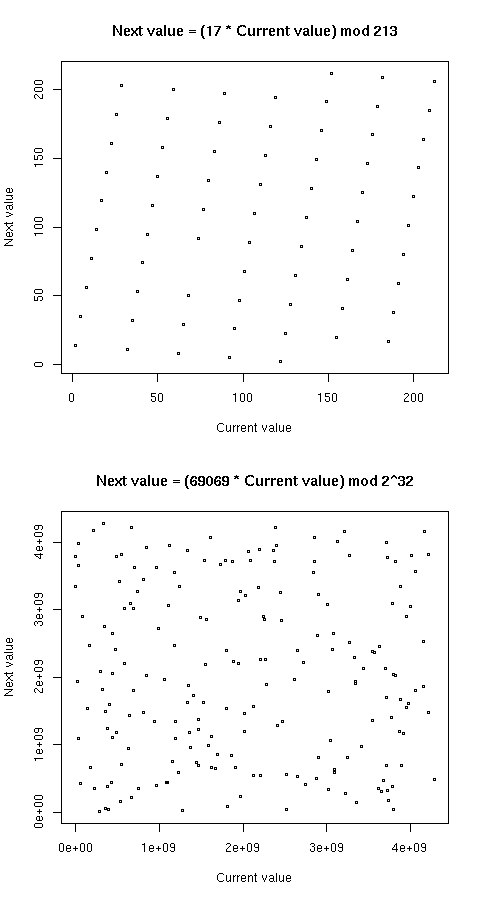
\includegraphics[height=6in]{computerIntro/images/cong.png}
\caption{For each scatter plot, two hundred values, $x_1$, $x_2$,
  \ldots, $x_{200}$ are generated according to the congruential
  method.  The points represent successive pairs of numbers,
  e.g. $(x_1, x_2)$, $(x_2, x_3)$, etc.  In the top plot, the method
  uses the algorithm $x_{n+1} = 17x_n~mod~213$, and the bottom plot
  uses the default values from one of R's generators, $69069x_n
  ~mod~2^{32}$.  The seed is $17$ in both cases. The first set of
  values show a stripy non-random pattern whereas the second set
  looks randomly scattered. }
\label{fig:congPlot}
\end{figure}


Several random number generators are offered in R. These are discussed
in Section~\ref{sec:repNum} as their designs are connected to the
representation of numbers in the computer.



\section{Understanding the R Language}\label{sec:languages}
When learning a programming language, one typically needs detailed,
specific information about particular syntactic structures such as how
to write a conditional statement or a loop or what are the inputs for
a particular function, but it is also important to have a broad ``big
picture'' understanding of the language.  Like with a human language,
one needs to become familiar with the rules of the language, but also
the vocabulary and the style and idioms that others use.  And for a
computer language, it helps and is important to understand the
rationale and logic that underlies how the language is understood by
the computer.  This helps you express computations properly and
understand why the computer may interpret the commands differently
from your expectations.

\begin{comment}
%this belongs in a different chapter
There are several sources of information about the R and S programming
languages that work at these different levels of specific information,
reference manuals and broad overviews.  In this chapter, we don't
attempt to provide all of these.  Rather, here we focus on trying to
understand the rationale of the language. We expect the reader to
explore the ideas interactively using the R environment as they read
this and do some experiments to see how the language works.  We have a
terrific, interactive medium with which we can hypothesize and test
characteristics.
\end{comment}

Finding out how R works and learning to think about how to express
computations in R will greatly simplify your work when using R. It is
good to take the time early on to learn a language and not simply use
it in a utilitarian, ad hoc manner.  And while R is a specific
language that you may or may not use extensively in the future, it is
important to realize that what you will learn when exploring R will be
generally applicable to many different programming languages that you
might use.  R is very similar to Matlab, and shares many of the same
concepts as Perl, Python, Java, C, and FORTRAN.  Although they are all
quite different, they also share important commonalities that are
essential when communicating about computations to others and to the
computer.

R is both an interactive and interpreted language.  By interpreted, we
mean that we can give an instruction and immediately have it
evaluated.  Then, we can give another command.  In other,
non-interpreted languages, we must write an entire program made up of
a sequence of commands that are specified before we run the program.
We have to order the instructions and take account of different
possibilities.  Once the program is running, we cannot change the
commands.  All we can do is either wait for it to complete or
terminate it and re-run it with the commands altered or different
inputs.


Interactivity is very important for statisticians.  We need to be able
to visualize data, look at numerical summaries and the output from
fitting a model, or subsetting the data based on previous observations
and then decide what to do next.  This process has been given the
name, Exploratory Data Analysis, or EDA for short.  It is a highly
iterative process where we attempt to let the data direct us as to
what to do next.  We try different things as we go along different
branches or paths. Sometimes these lead to useful insights that we
want to report. At other times, they verify that certain assumptions
are justified, or they suggest trying different methods to better
understand the data.  The ability to dynamically specify what we want
to do next is important.  R then allows us to combine commands into a
script or ``program'' that we can re-run on new or different data to
recreate our analyses.  This is often termed \textit{batch}
programming since we are doing several commands in a single run. This
combination of interactive commands and running scripts in a batch
gives us the best of both worlds: we use interactive facilities during
exploration, and programming facilities when the exploration is more
``complete''.


\section{Digital Information}\label{sec:digital}
A computer is a general purpose information processing machine.  The
information it can process could be a movie on DVD, a collection of
photos on a CD, a Web page on the Internet, an Excel spreadsheet
stored on a memory stick, or a plain text file on the computer's hard
drive.  All of these examples are digital because computers are
digital devices.

The smallest unit of information in a computer has just two states.
For example, CDs and DVDs are optical storage devices that use two
different levels of light reflectance to represent information.  Also,
memory cells in a computer are either charged or cleared, and magnetic
storage devices like the hard drive in a computer have areas that are
either magnetized or not.  These two states can be represented by the
binary digits 1 and 0.  Binary digits are the building blocks for all
information processing in computers.

The term ``bit'' is an abbreviation for binary digit. Interestingly,
it was a statistician from Bell Labs, John Tukey, who coined the term
in 1946. While information is made up of bits, we typically work
at the level of ``bytes'' and higher level entities.  A byte is a unit
of information built from eight bits.  The notion of a byte was first
used in encoding characters. For example, the 8 bits, $01000001$
encodes the capital letter \verb+A+.

\subsection{Characters}\label{sec:characters}
In order for digital devices (hard disks, CDs, DVDs, etc.) to process
and store text information we need a correspondence between bit
patterns and the symbols of a written language, which are called
glyphs.  ASCII (American Standard Code for Information Interchange)
was created in the early 1960s as a bit encoding for the English
alphabet. It uses seven bits to represent character glyphs.  For
example, $1000001$ represents the upper case \verb+A+, the glyph
\verb+B+ is coded as $1000010$, \verb+C+ is $1000011$ and so on.  The
eighth bit in an ASCII byte is typically set to zero, although
historically it was used for error checking.

Modern character encodings support many more characters, while also
typically remaining compatible with ASCII.  One example is Unicode.
It uses 16 bits to encode characters, rather than 7.  Unicode is an
industry standard designed to allow text and symbols from all of the
writing systems of the world to be consistently represented and
manipulated by computers.  The first 128 characters ($2^7= 128$) of
Unicode are compatible with ASCII.  See Table~\ref{tab:ASCII} for
examples of the ASCII and Unicode mapping from bits to glyphs.

\begin{table}
\begin{center}
\begin{tabular}{ccc|cc}
  \multicolumn{5}{c}{Binary Representations of Characters}  \\
Glyph & ASCII & UniCode & Glyph & Unicode \\
\hline
\# & 0010 0011 & 0000 0000 0010 0011 & \copyright & 0000 0000 1010 1001 \\
\$ & 0010 0100 & 0000 0000 0010 0100 & \ae  & 0000 0000 1110 0110 \\
A & 0100 0001 & 0000 0000 0100 0001 & $\Delta$ & 0000 0011 1001 0100\\
a & 0110 0001 & 0000 0000 0110 0001 & $\alpha$ & 0000 0011 1011 0001\\
\hline
\end{tabular}
\caption{A few examples of the mapping from glyph character to ASCII
  and Unicode.  ASCII uses 7 bits to represent characters (with the
  eighth bit typically set to 0) and Unicode uses 16. The ASCII and
  Unicode mappings are compatible for the $2^7 = 128$ ASCII
  characters.  The two glyphs on the bottom right of the table (the
  Greek letters, capital delta and lower case alpha) do not have
  encodings in ASCII. }
\label{tab:ASCII}
\end{center}
\end{table}


The table on the How Stuff Works Web page
(Figure~\ref{fig:HowStuffWorks}) and the plain text table in
Table~\ref{tab:chip} are both encoded in ASCII, while the Excel
spreadsheet (Figure~\ref{fig:csvExcel}) stores the data in a
different encoding.  Although the information is essentially the same
in all three contexts, there are important differences between them.
These are described in Section~\ref{sec:electronicFiles}.


\subsection{Representation of Numbers}\label{sec:repNum}
The original data used to create the plot in Figure~\ref{fig:chip} may
have come from a plain text table, but when it is read into R, it is
stored in a very different format.  For example, when we multiply the
most recent two values of \SVariable{Speed} by $1000$, this
multiplication is not being performed on ASCII characters.  R is
storing these numbers in a different format than ASCII or Unicode, a
format that is conducive to performing arithmetic computations.

The main system of mathematical notation today is the decimal system,
which is a base-10 system.  The decimal system uses 10 digits, 0, 1,
2, 3, 4, 5, 6, 7, 8, 9, and numbers are represented by the position of
these digits. For example, the numbers 200, 70, and 8 represent 2
hundreds, 7 tens, and 8 units, respectively. Together, they make the
number, 278.  Clever people who designed and developed computers
realized that it is more efficient if we take advantage of the on-off
nature of bits, and represent numbers using base 2 rather than decimal
(base 10).  To understand how to do this, we express the decimal
representation of a number such as $278$ with powers of $10$ as
follows:
\begin{equation}
278 = (2 \times 10^2) + (7 \times 10^1) + (8 \times 10^0).
\end{equation}
The binary system, simply uses powers of two for the positions of the
digits $0$ and $1$. For example, the binary number $1101$ in base $2$.
\begin{eqnarray*}
1101_{2} & = & (1 \times 2^3) + (1 \times 2^2) + (0 \times 2^1) + (1 \times 2^0) \\
     & = & (8) + (4) + (0 ) + (1 )  = 13_{10}
\end{eqnarray*}
The equation shows that $1101$ in base 2 is equivalent to the number
$13$ in base ten.  Note that the subscript $2$ on the number 1101
tells us that the number is being represented in base-2 rather than
base-10. This representation in terms of powers of $2$ shows how to
convert numbers from base-2 into base-10 (see Figure~\ref{fig:base2}).

\begin{figure}
\begin{center}
\begin{tabular}{l|cccccccc|r}
    \multicolumn{10}{c}{$8$-digit Binary Number}  \\
     \hline
 Value & $2^7$ & $2^6$ & $2^5$ & $2^4$ & $2^3$ & $2^2$ & $2^1$ & $2^0$ \\
 \hline
  Position & $7$ & $6$ & $5$ & $4$ & $3$ & $2$ & $1$ & $0$ \\
\hline
  Base $2$ &   0 & 0  & 1 & 1 & 0 & 0 & 0 & 1 & $00110001$\\
\hline
 
 Base $10$  & 0 & 0  & 32 & 16 & 0 & 0 & 0 & 1 & $49$ \\
 \hline
\end{tabular}
\end{center}

\caption{The 8-digit binary number $00110001$ is equivalent to the
  2-digit decimal number $49$.  To see this, think of each position in
  the 8-digit number as representing a power of $2$, from $2^0$ to
  $2^7$. For a particular position, say the fifth position from the
  right, there appears a $1$ in the number $001[1]0001$ to indicate
  one $2^4$, or one $16$. The decimal equivalent of the binary number
  is then the sum of the corresponding decimal values for each
  position that contains the digit $1$.}
\label{fig:base2}
\end{figure}

When we work with integers or whole numbers, we know that there are
infinitely many of them.  However, the computer is a finite state
machine and can only hold a finite amount of information, albeit a
very, very large amount.  The solution that most computers implement
uses a fixed number of binary digits to represent an integer.  Then
computations can be done on the chip itself rather than in software
and be much, much faster. Most software offer the option of storing
integers using $1$, $2$, or $4$ bytes.  With $4$ bytes, integers from
$0$ to $2^{32} - 1 = 4,294,967,295$.  If we want to represent positive
and negative integers, then one of the bits must be used for the sign
and the remaining bits are used to represent the absolute value of the
integer.

If we need to compute with larger numbers, fractions, or real numbers,
then the computer represents these numbers using scientific notation.
Recall that a number such as $2.3$ can be represented via scientific
notation as $2.3 \times 10^0$, as $0.23 \times 10^1$, as $23 \times
10^{-1}$, etc.  That is, there is not a unique representation, unless
we settle on a convention such as: the mantissa must have exactly one
non-zero digit before the decimal point.  In our example, that means
we settle on $2.3 \times 10^0$.  This unique representation of a real
number has four components: the sign (+1) in this example, the
mantissa (2.3), the base (10), and the exponent (0).  The IEEE
(Institute of Electrical and Electronic Engineers) single-precision
floating point representation uses 32 bits, with one bit for the sign,
23 bits for the mantissa, and eight bits for the exponent.  Since the
leading digit of the mantissa will always be 1 in our base-two
representation, we need not store it.  In double-precision floating
point, we typically use 11 bits for the exponent and 52 bits for the
mantissa.  So the exponent has $2^{11}$ or 2048 possible values.  For
11 bits, the possible (signed integer) values for the exponent
range from $-1022$ to $1023$ with the remaining two values being
reserved for special cases.


Now with this understanding of the representation of numbers in a
computer, we can continue our discussion of random number
generation. Several random number generators are offered in R.  One is
based on the ``Super-Duper'' package of Marsaglia.  This generator
produces two 32-bit integer pseudo-random numbers.  One uses 
the congruential method with $a = 69069 $ and $ b = 2^{32}$, and produces
$2^{30}$ unique numbers before repeating.  The second uses the 32-bit
Tauswirthe generator, which has a period of $4,292,868,097$ for most
seeds. These two numbers are combined using the exclusive-or operation
on their 32 bits, and the resulting number is then divided by$2^{31}$
to produce a number between 0 and 1.  In R, the seed for the random
number generator is stored as an integer vector in the variable called
\SVariable{.Random.seed}.  There are several R functions that use this
internal generator to get independent random samples from probability
distributions other than the uniform on $[0,1)$. One example is the R
function \SFunction{rnorm}, the pseudo-random normal generator.


\subsection{Colors}
As a final example of binary data, consider the colorful images a
computer can render on its display.  The image is made of many pixels
or points, and each pixel is typically represented using the RGB (Red
Green Blue) color model.  The RGB model is based on the three kinds of
photoreceptor cells in the eye, where the pixel is represented in the
computer as a combination of intensities of these three colors. For
each color, 8 bits, i.e. one byte, represents the range of the color
to display. So RGB uses 24 bits (3 bytes) to represent colors.  The
minimum intensity for each of the three colors is $00000000$ and the
maximum is $11111111$.  For example, full intensity red is ($11111111$
$00000000$ $00000000$), and full intensity green and blue are
similarly defined. Other colors are made from combinations of these
three.  Full intensity yellow is ($11111111$ $11111111$ $00000000$),
cyan is a combination of full intensity green and blue ($00000000$
$11111111$ $11111111$), and chartreuse is ($01111111$ $11111111$
$00000000$). Black is the absence of red green and blue, and white is
the full intensity of all three.  With this system, there is the
possibility of creating $2^{24}$ color combinations, which is more
than $16$ million combinations of hue and intensity.  Most of us
cannot distinguish by eye more than a few hundred colors!


\section{Electronic Files}\label{sec:electronicFiles}
A ``plain text'' document such as the table in Table~\ref{tab:chip} is
a collection of characters that correspond to printed lines on a
piece of paper.  In a computer this information is contained in a
file, which is simply a sequence of bytes in a format such as ASCII or
Unicode.  A plain-text file can be opened and read by a plain-text
editor such as Emacs, Notepad, and TextEdit.  These editors are
examples of software capable of reading and displaying files that
consist of ASCII or Unicode characters. The editor understands the
meaning and internal layout of information in a plain-text file,
presents it to the user as a document, and enables her to edit the
information.  Now we see that the plain text table of chip data in
Figure~\ref{fig:csvExcel} is simply a collection of ASCII characters
in a file.

Other file formats are also text files, that adhere to more specific
rules which allow them to be used for specific purposes.  For example,
an HTML file that is displayed in a Web browse is also a plain-text
file.  However, it contains special markup that instructs the browser,
e.g.  Opera, FireFox or InternetExplorer, how to display the file
contents.  The markup is plain text, and it appears between angle
brackets.  For example, \verb+<h1>+ denotes a large header, \verb+<b>+
tells the browser to make the text boldface, and \verb+<p>+ denotes a
paragraph.  Given the markup, the browser determines how to display
the content. The HTML table rendered in Figure~\ref{fig:HowStuffWorks}
is again a plain text file, but with special characters that the
browser knows how to interpret in order to render it with particular
shape, background color, type face, etc.  A small piece of this file
is shown below.

{\footnotesize{
\begin{verbatim}
<p>
The following table helps you to understand the differences between 
the different processors that Intel has introduced over the years.
</p><p>
</p><center>
<table width="430" cellspacing="0" 
cellpadding="3" border="1" bgcolor="lightyellow">
<tbody>
<tr>
 <td><font size="-1" face="arial,helvetica">
  <strong><center>Name</center></strong></font></td>
 <td><font size="-1" face="arial,helvetica">
  <strong><center>Date</center></strong></font></td>
 <td><font size="-1" face="arial,helvetica">
  <strong><center>Transistors</center></strong></font></td>
 <td><font size="-1" face="arial,helvetica">
  <strong><center>Microns</center></strong></font></td>
 <td><font size="-1" face="arial,helvetica">
  <strong><center>Clock speed</center></strong></font></td>
 <td><font size="-1" face="arial,helvetica">
  <strong><center>Data width</center></strong></font></td>
 <td><font size="-1" face="arial,helvetica">
  <strong><center>MIPS</center></strong></font></td>
</tr>
<tr>
 <td><center><font size="-1"
  face="arial,helvetica">8080</font></center></td>
 <td><center><font size="-1"
  face="arial,helvetica">1974</font></center></td>
 <td><center><font size="-1"
  face="arial,helvetica">6,000</font></center></td>
 <td><center><font size="-1"
  face="arial,helvetica">6</font></center></td>
 <td><center><font size="-1" 
  face="arial,helvetica">2 MHz</font></center></td>
\end{verbatim}
}}

As another example, a CSV file is also a plain-text file where the
values in a line of text are separated by commas (CSV stands for
Comma-Separated Values). This special structure enables spreadsheet
programs, such as Excel and Gnumeric, to read and display the contents
in a row and column format where each line of text is a row, and the
values between commas in a line of text are placed into columns in the
row of the spreadsheet.

Many file formats, have a published specification that describes
exactly how the content is to be encoded.  This information can be
used to develop software for working with files in the described
format. However, some file formats are proprietary, and so not
released to the public.  The formats for the Microsoft Office Suite,
e.g. Excel and Word, are such examples.  An Excel spreadsheet is not
a plain-text file; it contains special instructions that describes how
to display the data, e.g. column headings, font size, bold face, etc.
The Excel spreadsheet program understands this markup in order to
properly display and edit the spreadsheets.

On the other hand, the portable document format (PDF) is an open
format developed by Adobe Systems to represent documents in a
universal manner.  A PDF file can be displayed and printed no matter
which software was used to create the corresponding document, whether
it includes text, graphics, or images, and regardless of the device
used to display it (e.g. the type of printer).  It is a subset of
PostScript encoding for generating layout and graphics, and it allows
fonts to be defined and included in the document.


\begin{comment}
\begin{figure}
\begin{center}
\begin{tabular}{c}
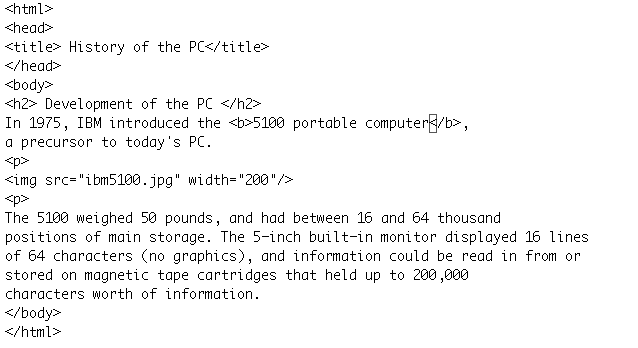
\includegraphics[width=5in]{computerIntro/images/htmlScreenshot.png}
\\
\\
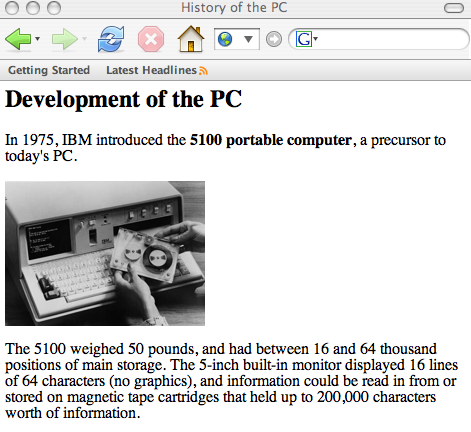
\includegraphics[width=5in]{computerIntro/images/browserScreenshot.png}
\end{tabular}
\caption{The plain text file (top - view from a plain-text editor)
  includes Hypertext Markup (HTML) which a browser software such as
  Firefox can read and display (bottom).  By simply resizing the
  browser window the line-breaks in a paragraph of text can change.
  Note that the jpeg image is not contained in the html file, only a
  reference to it.}
\label{fig:htmlBrowser}
\end{center}
\end{figure}
\end{comment}

\subsection{Identifying files}
Different file formats are designed to store different kinds of
digital information, such as documents, images, videos, and music. The
computer needs to be able to understand that a particular collection
of bytes represents a text document, an image, or a musical recording
in order to properly display it, edit it, print it, or play it.
Naming conventions have been established to make it simpler for
software to identify a file's format.  The file-name extension is
tacked on to the end of a file's name, and consists of a period
followed by a few letters (usually three) that identify the format.
For example, a plain text file will have a file extension of ``.txt'',
a CSV file will end with ``.csv'', a PDF file ends ``.pdf'', an HTML
file has either the extension ``.html'' or ``.htm'', an Excel
spreadsheet ends with ``.xsl'', and a Microsoft Word document ends
with ``.doc''.  Note that this handy convention can be ignored or
circumvented because it is possible to rename a file to a different
extension or to drop the extension without changing the contents of
the file.

Some file formats use a ``signature'' inside the file in order to
determine how to interpret the bytes of information. For example, the
beginning of a PNG file contains information that identifies it as a
PNG formatted image.  That is, the file begins with an 8-byte
``signature'', which contains the letters ``PNG'' and 2 newlines,
among other things.  If displayed in a plain text editor, it appears
as follows.
\begin{verbatim}
  ~IPNG^M
  ^Z
\end{verbatim} 
Once a program recognizes that a file has a PNG signature then it will
know how to interpret the rest of the file.  The PNG format for images
is a structured series of chunks.  Each chunk contains information on
its size and type, along with its data.  The chunk types are either
critical or ancillary, meaning that a program that encounters an
ancillary chunk can safely ignore it.  This chunk-based structure is
designed to allow the PNG format to be extended while maintaining
compatibility with older versions.

Another image format, GIF, has a signature that begins with the ASCII
representation of GIF87a or GIF89a.  Other formats also use a
signature or ``magic number'' that is stored inside the file to
uniquely identify its format.  Below are the signatures for postscript
and PDF formats, respectively.
{\footnotesize{
\begin{verbatim}
%!PS-Adobe-2.0
%%Creator: dvips(k) 5.92b Copyright 2002 Radical Eye Software
%%Title: DataTypes.dvi
\end{verbatim}

\begin{verbatim}
%PDF-1.4
3 0 obj <<
/Length 153
/Filter /FlateDecode
\end{verbatim}
}}

\subsection{Organizing Files}
Most computers organize files into hierarchies using folders or
directories. Each directory can contain an arbitrary number of files,
as well as other directories, which are referred to as
subdirectories. Subdirectories can contain files and subdirectories as
well. The system of directories and files makes a tree
structure. Figure~\ref{fig:tree} shows a tree representation of a file
system that has four levels. In this figure directories are
represented by squares and files by circles. The top of the tree is
the root directory, denoted by ``\verb+/+''. It contains all of the
files and directories.

Naming conventions for directories are the same as for files.  The
full path name of a file includes the hierarchy of directories that
contain the file.  For example, the full path name of the file
\File{X} within the directory \Directory{C} is \File{/A/C/X}, whereas
the full path name of the file \File{X} within directory \file{D} is
\File{/A/B/D/X}.  Files must be uniquely named, and although there are
three files with the name \File{X} in this directory structure, they
are uniquely named because their full path names are distinct.

\begin{figure}
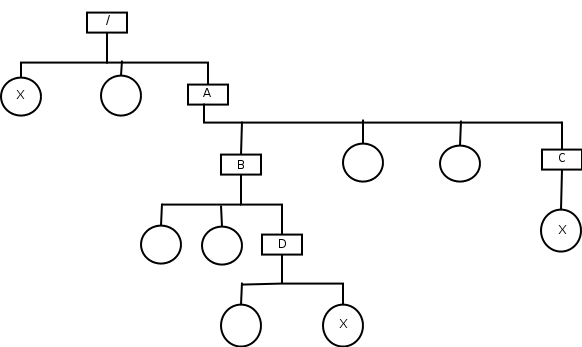
\includegraphics[width=5in]{computerIntro/images/fileTree.png}
\caption{A file system is represented here as a tree structure.  All
  of the symbols at the same level in the tree are in the same level
  of the directory structure.  Rectangular symbols represent
  directories and circles files.  Notice that there are three files
  with the name of $X$, however as they are in three distinct
  directories they are uniquely named (and so defined).  Their full
  pathnames, from top to bottom, are /X, /A/C/X and /A/B/D/X.}
\label{fig:tree}
\end{figure}

Files may also be referred to by relative path names.  For example,
relative to directory \Directory{A}, the file \File{X} in
\Directory{C} is referred to as \File{C/X}, and relative to
\Directory{A}, the file \File{X} in the top-level directory is
referred to as \File{../X}.  Here the two periods means go up one
level to \Directory{A}'s parent directory.  Users typically have a
default relative path, such as \Directory{/home/nolan/}, which can be
referred to as \verb+~+.  Hence \verb+~/+\Directory{A/C/X} is short
hand (a relative path name) for \Directory{/home/nolan/A/C/X}.

In the Windows operating system, pathnames use the backslash rather
than the forward slash.  Also, in general, file names must follow the
naming conventions required of the operating system. In most systems,
the forward slash and backslash characters, \verb+/+ and \verb+\+, are
forbidden in a name as they would be confused with directory
names. How systems handle upper and lower case varies.  For example
Unix file systems are usually case sensitive and allow user-level
applications to create files whose names differ only in the case of
characters. Whereas, Mac OS X preserves case when a file is named, but
is generally case insensitive.


\section{Components of a computer}\label{sec:components}
Most of us treat computers as black boxes that we provide input to and
get output from, and don't care about how they work. However, given
the implications of processing speed, memory, and storage on our
ability to perform scientific computations, it is good to understand
the basic structure of a computer so that we have a sense of its
limits, and so we can fix simple things and recognize potentially more
serious problems.

A computer is a general-purpose information processing machine.  For
example, the computer can display a movie for you to watch that is
stored on a DVD, or it can transfer a copy of an Excel file from a
memory stick to its hard drive for later computations.  There are many
ways to get information into a computer.  It takes input through
devices such as a keyboard and mouse, and it receives information via
a microphone or a stylus and tablet.  The keyboard, mouse, microphone,
and tablet are all known as input devices.  Information is also input
to a computer via removable storage devices, such as a compact disc
(CD), digital versatile disc (DVD), and memory stick, and from
permanent storage devices, such as a hard disk.  The Internet is yet
another means for the computer to obtain information.

The computer also gives us information.  That is, we receive
information from a computer via output devices.  We can look at a
photo on a monitor, read a news article printed to a printer, and
listen to music on the computer's speakers. The computer can also
store information on external output devices; e.g. it can store
digital information on a hard disk; it uses a CD or DVD drive to write
information to CDs and DVDs; and it can send information over the
network to another storage device.

Aside from these input and output devices, the ``guts'' of the
computer that processes information are in the ``box'', i.e. the
laptop, desktop ``tower'', or rack-mounted box.  Inside this box there
are just a few components -- the motherboard, Central Processing Unit
(CPU), Random Access Memory (RAM), hard drive and disk drive.

\begin{figure}
\begin{center}
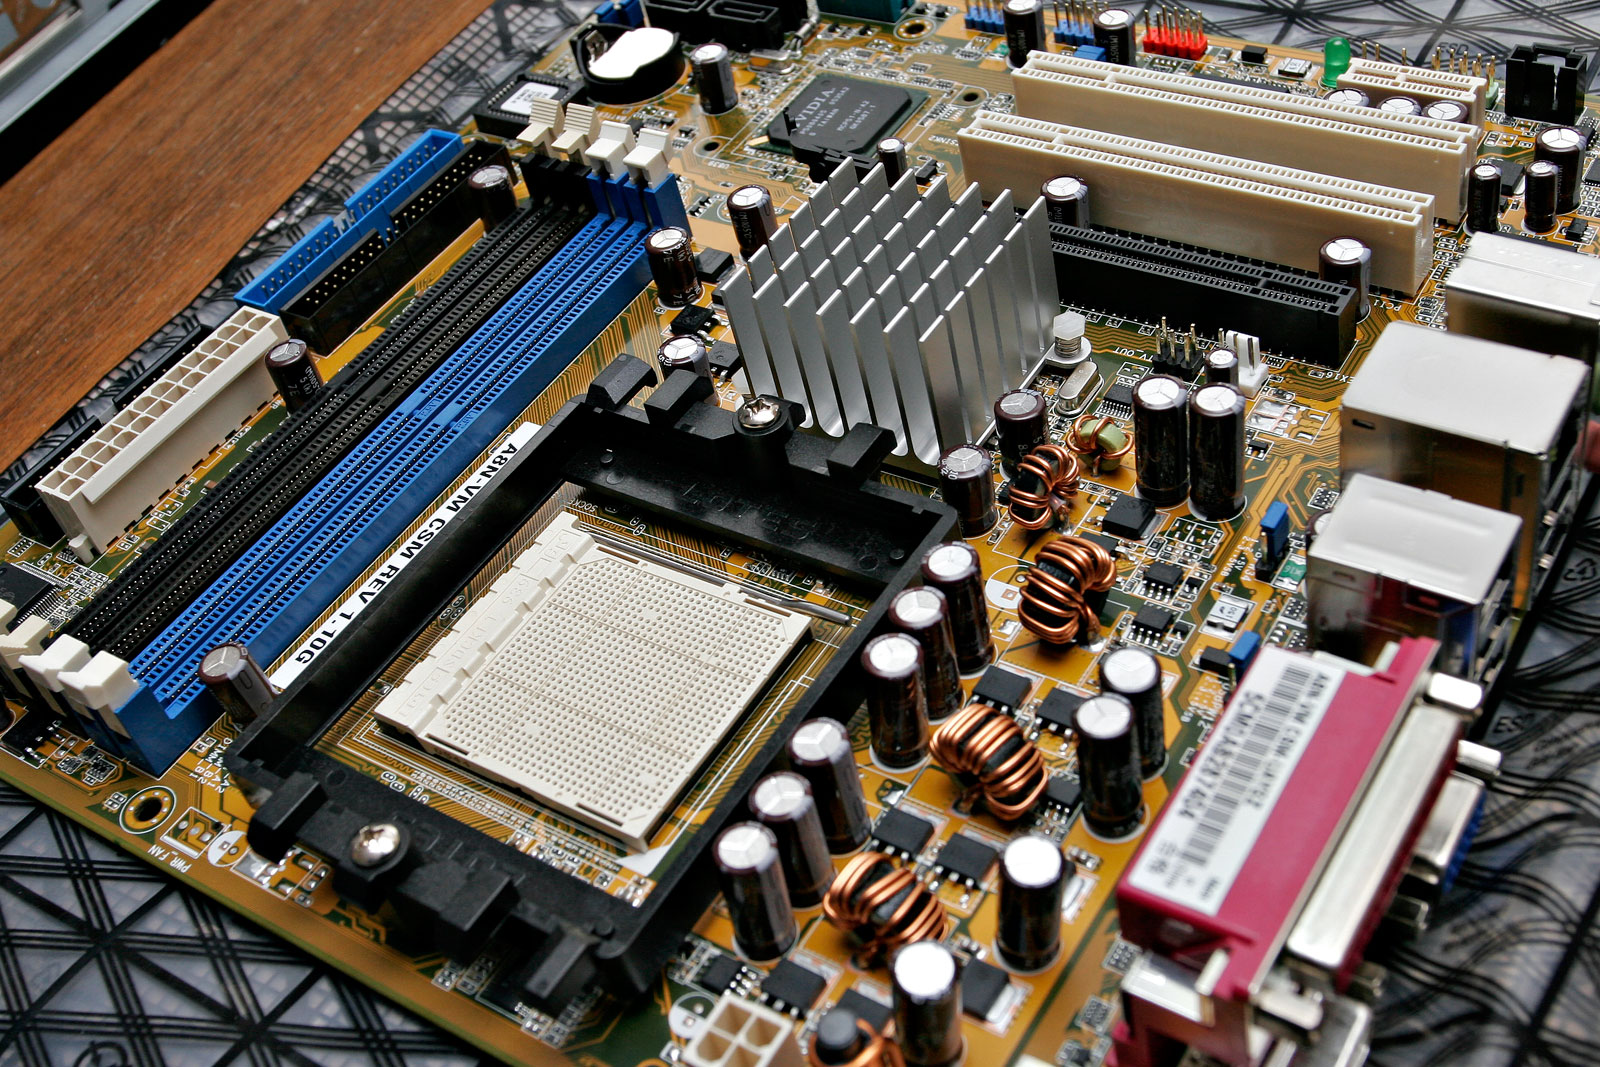
\includegraphics[height=3in]{computerIntro/images/motherboardHiRes.jpg}
\caption{The motherboard of a computer.}\label{fig:thinkpad}
\end{center}
\end{figure}

\subsection{Motherboard} The \Key{motherboard} is the physical board
that connects the internal components and also provides connectors
known as ports for the external devices.  The chips for the CPU are
plugged in or soldered to the motherboard, memory cards and video
cards are plugged in via slots, and a printer, keyboard, and internet
connection are made available via ports on the motherboard.  In other
words, the motherboard provides a common electrical and communication
system for all of the devices and internal components.  It contains
several layers that are sandwiched together.  The layers responsible
for the communication system carry data via busses, while other layers
carry voltage for the common electrical system.

\subsection{Central Processing Unit} The \Key{CPU}, also called the
microprocessor chip, is the heart of the computer.  The chip is an
integrated circuit made of transistors and capacitors that hold a
complete computation engine.  This computation engine consists of
fairly simple digital logic techniques -- it can add, multiply, fetch
a value from memory, store a value into memory, and do several other
primitive things.  More complex computations can be done in software
by combining different primitive instructions to get new, higher-level
commands.

Clock cycles are used to coordinate the actions of the transistors, so
how fast an instruction is performed depends on the chip's clock
speed. The Pentium 4 microprocessor is very fast; its clock speed is
over 3 GigaHertz (see Table~\ref{fig:HowStuffWorks}) -- that's over
three billion clock cycles per second.  Different chip designs allow
different instructions to execute natively on the circuit.  For
example, the instruction set for a Pentium chip is different from that
of the Mac G4 processor.  The G4 processor is based on RISC (Reduced
Instruction Set Computer) technology, while the Pentium 4 uses CISC
(Complex Instruction Set Computer) technology.  RISC technology has
fewer commands than CISC (about 50 compared to a few hundred), but
these commands require fewer clock cycles per instruction. This means
that the RISC processor can typically carry out more instructions in
one clock cycle than a CISC processor, e.g. the G4 can complete one
double-precision calculation every clock cycle, while the Pentium 4
cannot.  For this reason, although the G4 processor runs at only about
half the clock speed of the Pentium, clock speed does not provide a
straight forward comparison of their computational speeds.  In
addition, other factors affect computational speed such as the number
of transistors on a chip, the bus speed for moving data, and memory
size.



\begin{comment}
\begin{table}
\begin{center}
\begin{tabular}{lrrrrrr}
\textbf{Name} & \textbf{Date} & \textbf{Transistors} & \textbf{Microns} & \textbf{Clock speed} & \textbf{Data width} & \textbf{MIPS}\\
\hline
8080 & 1974 & 6000 & 6 & 2 MHz & 8 & 0.64\\
8088 & 1979 & 29000 & 3 & 5 MHz & 16 & 0.33\\
80286 & 1982 & 134000 & 1.5 &  6 MHz & 16 & 1\\
80386 & 1985 & 275000 & 1.5 & 16 MHz & 32 & 5\\
80486 & 1989 & 1200000 & 1 & 25 MHz & 32 & 20 \\
Pentium & 1993 & 3100000 & 0.8 & 60 MHz & 32 & 100\\
PentiumII & 1997 & 7500000 & 0.35 & 233 MHz & 32 & 300\\
PentiumIII & 1999 & 9500000 & 0.25 & 450 MHz & 32 & 510\\
Pentium4 & 2000 & 42000000 & 0.18 & 1.5 GHz & 32 & 1700 \\
Pentium4x & 2004 & 125000000 & 0.09 & 3.6 GHz & 32 & 7000\\
\end{tabular}
\caption{The Intel microprocessor has become much faster, smaller, and
  more powerful in the past thirty years, as seen by several measures.
  From left to right, these measures are the number of transistors on
  the chip, the width in microns of the smallest wire on the chip, the
  clock speed (number of cycles per second), the number of bits used
  for addressing data in RAM, and millions of instructions per second.
  The plot in Figure shows a comparative picture of the changes in
  these variables over time. These data are from
  \texttt{http://computer.howstuffworks.com/microprocessor1.htm}}
\label{tab:chip}
\end{center}
\end{table}
\end{comment}
   

\subsection{Memory}  
For the microprocessor to perform an instruction, the information it
requires is brought to the chip and placed directly in its
registers. The inputs to and the outputs from an instruction are very
simple values such as numbers, logical values, etc. They move to and
from the registers to a local piece of memory on the chip for
immediate reuse. The CPU has limited space in this memory cache for
storing values for the next command, and when the cache gets full,
this information is moved to bigger areas of memory, namely Random
Access Memory (RAM).

\subsubsection{Random Access Memory}
The read/write speed of RAM is much faster than a hard drive, and
unlike the technology of the hard drive, RAM technology is geared
toward accessing small pieces of data at a time.  For these reasons,
it is much faster to have the data that the CPU needs for a
computation available in RAM rather than leaving it on a storage
device such as the hard disk or a DVD.  (Random access memory is
considered ``random access'' because any memory cell can be accessed
directly if you know its location.)

Similar to a microprocessor, RAM is a chip, which is an integrated
circuit made of transistors and capacitors. In its most common form,
dynamic RAM, a transistor and a capacitor are paired to create a
memory cell.  The transistor acts as a switch that lets the cell be
read or changed. A capacitor is like a small bucket that stores
electrons. However, capacitors are leaky, and in a matter of a few
milliseconds a full capacitor loses its charge.  Therefore, the
``full'' capacitors must be constantly recharged. When the computer is
turned off, the charge in the capacitors is lost, and the contents of
RAM is gone.

In addition to this volatile dynamic RAM, a computer often has static
RAM as well.  This supply of memory has a direct connection to the
CPU, and never has to be refreshed, which makes it significantly
faster than dynamic RAM.  However, because it has more parts, a static
memory cell takes up a lot more space on a chip than a dynamic memory
cell, and that makes static RAM a lot more expensive.

Computers are often classified by the number of bits they can process
at one time, as well as by the number of bits used to represent
addresses in their main memory (RAM).  The number of bits used by a
computer's CPU for addressing information represents one measure of a
computer's speed and power.  Computers today often use 32 or 64 bits
in groups of 4 and 8 bytes, respectively, in their addressing.  A
32-bit processor, for example, has 32-bit registers, 32-bit data
busses, and 32-bit address busses. This means that a 32-bit address
bus can potentially access up to $2^{32} = 4,294,967,296$ distinct
memory cells (or bytes) in RAM. Whereas a $64$-bit processor can
access $2^{64}$ memory cells, which means the computer will be faster
with computations that require a lot of memory. Memory and data
capacity are commonly measured in kilobytes ($2^{10} = 1024$ bytes),
megabytes ($2^{20} = 1,048,576$ bytes), or gigabytes ($2^{30} =
1,073,741,824$, about 1 billion bytes). So a 32-bit address bus means
that the CPU has the potential to access about 4 GB of RAM.

\subsubsection{Virtual Memory}  
When RAM gets full, information is moved from RAM to a temporary area
on the hard drive, called the swap area or virtual memory.  The
computer manages the memory needed for computations.  It looks at RAM
for areas that have not been used recently by the CPU and copies these
areas onto the hard disk in an area set aside for temporary
storage. This frees up space in RAM to load new data. The temporary
area on the hard drive is called virtual memory because the copying
described here happens automatically and makes your computer act like
it has unlimited (or really large) RAM space. However, virtual memory
is much slower than RAM.  When performing computations there is a
trade-off between RAM and speed: the more information we hold around,
i.e. the more memory we use, the faster computations are.

\subsubsection{Read-only Memory} 
Read-only memory (ROM), also known as firmware, is an integrated
circuit programmed with specific data when it is manufactured.  This
memory is used to store the initial instructions the computer needs to
start. When we turn on a machine, it ``boots'' up which means that it
bootstraps itself into activity. It does this bootstrapping using its
BIOS (Basic Input/Output System) located in ROM.  The BIOS
instructions do things like test the hardware of the machine. In
general, it provides a very low-level interface to the different
components of the machine and the peripherals.  This bootstrapping
step initializes the components and gets the machinery into working
condition, and then tries to find the operating system to which it
will pass control.  This operating system might be Windows, MacOS X,
Linux, BSD or some other system.  It might be located on (one of) the
hard drive(s), on a CD or even on another machine.


\begin{comment}
  ??With the tremendous growth in information stored on disks,
  computer scientists have started to conduct studies of the
  reliability of disk drives. Recently, Google engineers studied their
  disk drive population where they examined disk failures for
  approximately 100,000 hard drives over an eight month period. They
  found some surprising results.  For instance, it appears that
  failures do not correlate with temperature.  Also they found that
  while scan errors are associated with increased chance of disk
  failure, the detection of the first scan error affects the chance of
  survival differently for newer drives in comparison to older
  drives. The younger drives, the chance of failure increase sharply
  within the first month after the scan error is detected and then
  flatten out, whereas for the older drives, the failure rate steadily
  increases throughout the observed eight months. (See
  Figure~\ref{fig:googleDriveFailure}.)

\begin{figure}
\begin{center}
PUT FIGURE HERE
\caption{The survival rate of disk drives in the eight months after
  the first scan error.  The disk drives are grouped according to the
  age at the time of the scan error. The curve for the younger drives
  ($0-8$ months old) drops sharply in the month after the first scan
  error and then levels out at about 90\%.  In comparison, the drives
  that are at least two years old, drops even more sharply in the
  first month and then continues to decline
  steadily.}\label{fig:googleDriveFailure}
\end{center}
\end{figure}
\end{comment}


\subsection{Operating System} The operating system, and specifically
the kernel, is essentially a regular application that manages the
resources of the machine. The kernel is run when the operating system
is started and it can start other applications, allocate resources to
these applications and basically coordinates access to the disks, file
systems on the disks, network connectivity, screen, memory, and so on.
At the simplest level, an operating system does two things:
\begin{itemize}
\item It manages the hardware and software resources of the computer
  system.  These resources include such things as the processor,
  memory, disk space, etc.  The operating system makes sure that each
  application gets the necessary resources and shares these resources
  with the other applications running on the computer.

\item It provides a stable, consistent way for applications and users
  to deal with the hardware without having to know all its details.
  That is, the operating system provides a consistent application
  interface and user interface, no matter what particular type of
  computer it is running on.
\end{itemize}

A consistent application program interface (API) allows a software
developer to write an application on one computer and have a high
level of confidence that it will run on another computer of the same
type, even if the amount of memory or the quantity of storage is
different on the two machines.  Also, an operating system can ensure
that applications continue to run when hardware upgrades and updates
occur, because the operating system and not the application is charged
with managing the hardware and the distribution resources.


\subsection{Storage Devices}
Hard disks or disk drives store information magnetically on flat disks
sometimes called platters.  These disks spin very quickly as a
read/write head moves from the center to the edge of the disk finding,
reading, and writing, information.  In this way, magnetic storage can
be easily erased and rewritten, yet the disk can store information for
many years.

A compact disk stores and reads information using optical or laser
technology rather than magnetism. The CD is a plastic disk with a
smooth reflective layer on top of a photosensitive dye.  Information
is written on a CD, or burned on, with a laser that heats the dye
layer and turns it dark. The CD is read by another laser that tracks
the reflection of its beam.  The light from the read-laser reflect
back to the laser at different levels according to whether or not the
reflective layer is obscured by the darkened dye or
not. Alternatively, CDs can have information stamped on them.  These
CDs have bumps and flat regions stamped into the reflective surface;
similar to the photo-sensitive dye, the bumps reflect the light
differently than the flat spots. DVDs are like CDs but with a much
larger storage capacity.


\subsection{A Bit of History}
In 1975, IBM introduced the 5100 portable computer
(Figure~\ref{fig:5100Thinkpad}), a precursor to today's PC. The 5100
weighed 50 pounds, and had between 16 and 64 thousand positions of
main storage. The 5-inch built-in monitor displayed 16 lines of 64
characters (no graphics), and information could be read in from or
stored on magnetic tape cartridges that held up to 200,000 characters
worth of information (that's about the equivalent of all the letters
in the first three chapters of this book).  Depending on its features,
the 5100 cost from nine to twenty thousand dollars (1975 dollars).  A
little over fifteen years later, IBM launched its Thinkpad series
(Figure~\ref{fig:5100Thinkpad}).  Like the 5100, these notebooks have
a keyboard, monitor, and storage drive built into the main unit, but a
Thinkpad is a far smaller, more powerful machine than its
predecessor. For example, the 1$\times$10$\times$12 inch Thinkpad T41,
introduced in 2003, weighs only 5 pounds, has a 14-inch screen with
1024$\times$768 color pixels, and cost only \$1,500-\$3,000, depending
on the configuration. The memory available for the T41 ranges between
256MB and 2GB, about 30,000 times that of the 5100. In place of a
tape-cartridge device, information can be stored on a CD, DVD, or a
40-80 GB hard drive. Other features include things we all expect in a
laptop these days, such as a touchpad with mouse buttons, battery with
four hours of life, and built-in antenna for connecting to the
Internet.

\begin{figure}
\begin{center}
\begin{tabular}{cc}
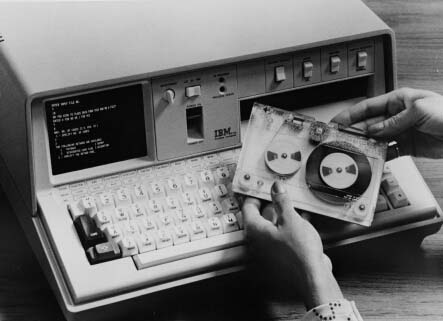
\includegraphics[width=3in]{computerIntro/images/ibm5100.jpg}
&
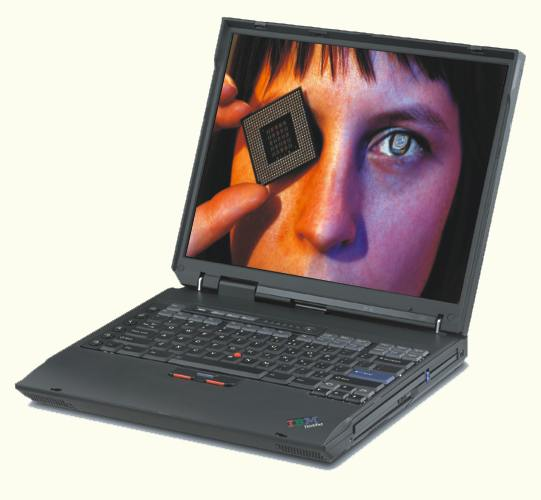
\includegraphics[height=2.2in]{computerIntro/images/ibmThinkpad.jpg}
\end{tabular}
\caption{The 5100 (left), introduced by IBM in 1975, was the precursor
  to the PC.  The keyboard, monitor, and tape drive were built into
  the unit.  Designed for engineers and scientists, it weighed about
  50 pounds and cost \$9,000 to \$20,000.  Thirty years later, IBM's
  Thinkpad laptop (right) also came with the monitor, keyboard, and
  storage device built-in.  However, it weighs only 5 pounds, has a
  hundred thousand times the memory, nearly a million times the
  storage capacity, and costs around \$2,000 in today's dollars.}
\label{fig:5100Thinkpad}
\end{center}
\end{figure}

According to the announcements at the time, the 5100 would ``put
computer capabilities at the fingertips of engineers, analysts,
statisticians and other problem-solvers.'' \footnote{IBM PC exhibit.
  http://www-03.ibm.com/ibm/history/exhibits/pc/pc$\_$2.html} Clearly,
the PCs and laptops of today have accomplished this claim and then
some.  By 2003, the year the T41 was introduced, IBM sold its 20
millionth ThinkPad. This dramatic change in computing power over the
past thirty years has indeed made a significant impact on scientific
computing. 


\begin{comment}This is an introduction to desktops, laptops, and
  mainframes; it is not an introduction to embedded computational
  devices in cars, cell phones, automated teller machines, etc.
\end{comment}


\section{Computing Languages}
The commands that we use in a programming language provide access to
complex operations.  They are built from primitive instructions that
reside on the computer chip.  These primitive instructions are
analogous to the axioms of mathematics, and programming languages
provide access to the more complex operations that are built from
these ``axioms''.  Like human languages, there are many computer
languages that have evolved in different communities with different
dialects.  These can be roughly categorized into low-level assembler
language, compiled languages, virtual machines, and interpreted
languages.  In addition there also point-and-click and drag-and-drop
interfaces to computing.


\subsection{Assembler} 
Assembler language is a very low-level, primitive language used to
specify sequences of CPU-level instructions to do a higher-level task.
The language is tied to the particular set of instructions available
on the CPU.  The assembler programmer has to do all the work,
specifying exactly what to do in the CPU's own language. For example
to perform a simple calculation such as $z = x + 3*y$ requires many
low-level instructions, such as
\begin{itemize}
\item Get value in address of $y$, put in register
\item Put 3 in register
\item Multiply, store result in register
\item Get value in address of $x$, put in register
\item Add, put result in register
\item Put result in address of $z$
\end{itemize}

The software written in assembler is often very fast to run, but on
the other hand it is slow to develop and maintain.  Most of us do not
want to worry about moving bytes in and out of CPU registers. The
high-level systems we use for working with data insulate us from the
representations of different types of numbers and from underflow and
overflow errors.  And this is where we want to be - using commands
that allow us to think in terms of the data and the statistical
problem on which we are working, and leaving the mapping of these
actions to the basic operations to the low-level computer
facilities. This is the general premise motivating programming
languages such as Fortran, C, Java, and much higher-level languages
such as S (R and S-Plus), Matlab, SAS, and other applications such as
Excel.

These languages allow people to express computations in a more human
readable and understandable way.  The instructions in these higher
level languages are translated by the language software to machine
code that the CPU can understand.

\subsection{Compiled languages}
One step above assembler are the C and Fortran languages.  Fortran
provides a higher-level mechanism to express computations involving
formulae and the language translates these formulae to machine
instructions. This is where the name Fortran comes from:
\textit{for}mula \textit{tran}slator.  The Fortran language has
evolved from Fortran 66 to Fortran 2000, which has increasingly modern
programming facilities. Because of the simplicity of the language, it
is quite fast and some argue that it is the most efficient language
for scientific computing. (This requires much greater specificity
about what efficiency means and also how to measure performance
appropriately.)  Fortran is useful, but it is clumsy and less well
suited to good software engineering than most other common languages.
However, it is very useful to be able to read and interact with
Fortran code because so much of the existing numerical software was
developed in Fortran.

The C language is a much richer language than Fortran and has been
used to implement operating systems such as Unix and Linux.  It has
been the language of choice for many years and is used widely in
numerical computing.  More recently C++ has become fashionable because
it offers many benefits over its close ancestor, C.  However, these
benefits are not without complexity.

Both Fortran and C are languages that are compiled.  In other words,
programmers write code and then pass it to another application - the
compiler - that turns it into very low-level machine instructions.
The result is an executable that can be run to carry out the
instructions.  Such executables are invariably machine-dependent,
containing machine-level operations that are specific to the machine
targeted by the compiler.  The same source code can be recompiled on
other machines, but this compilation step is necessary, and in many
cases, one must either modify the code for the new machine or be
conscious of the portability constraints when authoring the code.


\subsection{Virtual Machines}
Compiled languages, i.e. those requiring a compiler, are very
useful. Typically, the compilation step performs optimization
procedures on the programmer's code, making it faster by, e.g.,
looking at the collection of computations and removing
redundancies. Additionally, because compiled languages typically
require variable declarations in terms of scope and type information,
they can often catch programming errors before the code is run.  

\begin{comment}
%This appears earlier
There are disadvantages, however.  Using compiled languages, one
typically has to write an entire program before compiling it.  This
means that

\begin{itemize}
\item exploration and rapid prototyping of individual chunks is more
  complex or impossible. Specifically, it is much more difficult to
  incrementally create software by running individual commands.
\item one cannot typically alter the programming as it is running to
  correct errors or add functionality.
\end{itemize}
\end{comment}

The C++ language is in some sense an object-oriented extension of
C. It is a compiled language that allows for greater code reuse and
better software engineering for extensibility.  From our perspective,
C++ is still a low-level, compiled language that is analogous to C.

Java and C\# are very similar languages that one can categorize as
being simplified variations of C++ that promote the object-oriented
style of programming but without the complexity of C++.  They are also
compiled languages, requiring a separate compilation step.  Unlike C
and Fortran compilers, the Java and C\# compilers transform the
programmer's code into higher-level instructions targeted at what is
termed a Virtual Machine (VM).  The VM acts much like a computer,
processing the instructions, providing registers, etc. and generally
mimicking the actions of the low-level computer. This is done by
creating a version of the virtual machine for each computer
architecture (e.g. Powerbook, Intel *86, Sparc), but then allowing all
code for that virtual machine to run independently of what machine it
is running on. The virtual machine is a layer between the compiled
code and the low-level computer. And this makes the compiled code
(byte code) independent of the particular architecture and so makes it
portable without the need for recompiling.


\subsection{Interpreted languages}
Instead of compiling source code into machine code, other languages
read and interpret the code dynamically.  That is, the language has an
interpreter that parses and evaluates the code as it finds it, one
command at a time.  The interpreter is often called a Virtual
Machine. It emulates the real machine, providing software
implementation of the higher-level constructs we need.  For example,
loops and iterations; conditional execution and branching; and
variables.  The virtual machine is, for example, itself written in C
and compiled, but it can run arbitrary code for that language.  This
emulation makes interpreted languages generally slower than compiled
ones. Examples of interpreted languages include: Java, Perl, Python,
R, S-Plus, Matlab, Octave, and SAS. Java and Perl first create
``byte-code'' to speed up interpretation, although they still use a
virtual machine.

The acronym Perl stands for Practical Extraction and Report Language.
Perl is designed for text processing, and as such, it is extremely
fast at text manipulation.  The arcane constructs of the language make
it easy to create very terse programs. Although this may be beneficial
when programming, it tends to be challenging when debugging or reading
code a short time later.  Some dislike the language from a software
engineering perspective, but love it for its practicality.  Similar to
Perl in concept and purpose is the interpreted language Python.
Python is much more elegant than Perl because it was developed from an
object-oriented perspective, unlike Perl where the object-oriented
capabilities were added on. Python does not have as many add-ons as
Perl-yet.
% The syntax of the language uses white space to identify
``stanzas'' or blocks in the code.

The interpreted languages such as R, S-Plus, Matlab, and Octave are
aimed at a specific audience, e.g. statisticians, engineers, and they
provide higher-level functionality that the audience would find
useful. These are written in C and made available through libraries or
toolboxes of ``routines'' that build on the core language.  (C has
very few built-in functions that statisticians and engineers want.)
Thus the trade-offs for the slower speed are the higher-level
language, the specialized functionality, and portability.

\begin{comment}
\subsubsection{Java} Java is a language, a Virtual Machine Interpreter
and a collection of libraries.  The language object oriented, and is
similar to C++ in syntax, but without many of the error-prone elements
of C++ related to garbage collection and memory management.  Java
provides support for parallel processing with threads. It is a very
portable language, but requires a VM for each platform/Operating
System.  Java can be used in Web pages, and it provides secure
computations in distributed environment.
\end{comment}

R and S-PLUS have a nearly identical syntax that is
based on the $S$ language.  They were developed by and for
statisticians, and are constantly evolving as the large community of
researchers provide add-ons that bring new statistical methodology to
the users.  R and S-plus are the de facto standard for statistical
research and non-standard analyses.

As a simple comparison of R and the lower-level C language, imagine we
have a vector of numbers $x$. In C or C++, to get the sum of the
values in $x$, we write the following code.
\begin{verbatim}
double total = 0;
int j; int n;
double x;
for (j=0; j<n; j++){
    total += x[j];
}
\end{verbatim}
In comparison, in R, we write \RCode{sum(x)}.

Matlab is a commercial interpreted language designed for
engineers.  It is remarkably fast performing linear algebra and
numerical modeling algorithms.  Matlab is a simple, general
programming language, but it has little support for high-level
statistical concepts, such as models and categorical data.  Octave is
an open source language that is mostly compatible with Matlab.

\begin{comment}
\subsubsection{SAS}
Systems or environments like SAS provide either a batch or interactive
interface.  The interactive interface supports exploratory,
interactive data analysis, but it does not allow the programmer to
readily manage the intermediate results from each step and put them
into the next steps and generally branch in different directions.  The
BATCH system allows us to do interactive work in very coarse-grained
increments; run these sequence of commands on this data and produce
this output. Then, look at the output and write some more code. While
superficially this is the same sequence of steps in EDA that we might
do in R, the interface is much less convenient.
\end{comment}

\subsection{Excel and JMP}
The point-and-click, drag-and-drop interfaces like the one provided by
Excel and in SAS' JMP are very useful for specific tasks such as
editing values in cells, quickly creating plots, etc.  Managing
results and output from different tasks (e.g. regression, ANOVA,
summary statistics) across sheets can be hard work.  The visual
interface which is the thing that makes Excel, and graphical user
interfaces (GUIs) in general, convenient is a hindrance here.  While
we can put different results in their own worksheets, this soon gets
cluttered and we spend time navigating the tabs in the workbook.
Another complexity in this world of point-and-click for EDA is that
specifying precisely what we mean can be difficult.  In some cases, we
might want to customize a particular methodology when applying it to
data, or we might want to draw a plot slightly differently, or use a
data set that we derive in a complex way from the original source.  For
these common but non-standard situations, a sequence of dialogs
provided by a ``wizard'' can be frustrating.  It is tediously long,
especially if we are doing it several times with different subsets of
the data or different data sets that we wish to compare.  In addition
to the unnecessary repetitiveness, we also cannot specify everything
we may want to. The dialogs provide access only to the common
options. In the interest of keeping them simple, the designers have
identified what they believe are the important elements a user can
specify and change.  It is not possible for us to create our own
modifications of these tasks, or at least it is a major project to do
so.

